\documentclass{article}

\usepackage[final]{neurips_2022}
%\usepackage[UTF8]{ctex}

\usepackage[utf8]{inputenc}
\usepackage[T1]{fontenc}
\usepackage{hyperref}
\usepackage{url}
\usepackage{booktabs}
\usepackage{amsfonts}
\usepackage{nicefrac}
\usepackage{float}
\usepackage{amsmath}
\usepackage{amssymb}
\usepackage{amsthm}
\usepackage{algorithm}
\usepackage{algpseudocode}
\usepackage{microtype}
\usepackage{xcolor}
\usepackage{bm}
\usepackage{graphicx}
\usepackage{subfigure}
\usepackage{listings}
\usepackage{quantikz}
\usepackage{caption}
\usepackage{tikz}
\usetikzlibrary{trees}
\hypersetup{
  colorlinks=true,
  linkbordercolor=white,
}
\newtheorem{definition}{Definition}[section]
\newtheorem{theorem}{Theorem}[section]
\renewcommand{\algorithmicrequire}{\textbf{Input:}}
\renewcommand{\algorithmicensure}{\textbf{Output:}}

\title{Explicit Quantum Circuits for Block Encodings of Sparse Matrices: A Review and Exploration}

\author{%
  \large Zibo Ren \\
  \large \texttt{2200010626}
  \And
  \large Zixuan Yuan \\
  \large \texttt{2200010825}
}

\begin{document}

\maketitle

\begin{abstract}

  Efficiently constructing quantum circuits for block encodings of matrices is crucial for leveraging quantum linear algebra algorithms, which promise significant speedups for many computational problems.
  A block encoding is a technique where a matrix of interest is embedded within a larger unitary matrix, making it amenable to quantum computation.
  The realization of quantum advantage, however, heavily relies on the effective construction of these block encoding circuits, a task that presents considerable challenges, even when dealing with well-structured sparse matrices.
  This report reviews the work by Camps et al. \cite{EQC} on explicit circuit constructions for block encodings of certain well-structured sparse matrices.
  We delve into their proposed strategies, analyze their numerical demonstrations and reproduce their experiments.
  Furthermore, we explore potential avenues for original contributions and future research directions stemming from this work.
  We also provide implementations of the quantum circuits discussed in this paper in Python.

\end{abstract}

\section{Introduction}

Quantum linear algebra algorithms have emerged as a promising avenue to achieve exponential speedups over classical counterparts in solving fundamental computational problems such as solving linear systems, eigenvalue decomposition, and singular value transformation \cite{EQC}. At the heart of these algorithms lies the technique of \emph{block encoding}, which enables the embedding of non-unitary matrices into larger unitary matrices\textemdash a prerequisite for quantum computation. Formally, an $(\alpha, m, \varepsilon)$-block-encoding of a matrix $A \in \mathbb{C}^{N \times N}$ involves constructing an $(m+n)$-qubit unitary $U_A$ such that
\begin{equation}
  \|A - \alpha(\bra{0^m} \otimes I_N)U_A(\ket{0^m} \otimes I_N)\|_2 \leq \varepsilon
\end{equation}
where $N=2^n$. However, despite theoretical guarantees of algorithmic efficiency, practical implementations of block encodings remain challenging, particularly for structured sparse matrices\textemdash a critical class of inputs for applications in graph theory, differential equations, and machine learning.

Prior work on block encoding primarily focused on abstract oracle-based constructions, leaving explicit circuit designs largely unexplored. For instance, while quantum singular value transformation (QSVT) \cite{Gilyen2019} theoretically enables polynomial transformations of matrices via block encodings, its practical utility hinges on the explicit construction of quantum circuits for structured matrices. Camps et al. \cite{EQC} recently addressed this gap by introducing a systematic framework for constructing efficient quantum circuits for $s$-sparse matrices, which are matrices with at most $s$ nonzeros per column. Their approach decomposes the block encoding unitary $U_A$ into two components: (1) an oracle circuit $O_C$ that encodes the sparsity pattern of $A$, and (2) an oracle circuit $O_A$ that encodes the numerical values of nonzero entries. This explicit decomposition bridges the gap between theoretical algorithms and hardware-realizable implementations.

The significance of this work is twofold. First, for scaled $s$-sparse matrices $A/s$, the authors demonstrate circuits with gate complexity $\text{poly}(n)$, where $n$ is the qubit count, by leveraging controlled rotations and shift operators (e.g., implementing the mapping $\ket{j} \mapsto \ket{\text{mod}(j \pm 1, N)}$ for cyclic graph adjacency matrices) \cite{EQC}. Second, they extend their framework to symmetric stochastic matrices, enabling direct block encodings of Chebyshev polynomials $T_k(P)$ for quantum walks\textemdash a task previously hindered by scaling factors $1/s$ that degraded algorithmic efficiency. For example, their explicit construction of a quantum circuit for the block encoding of a $8 \times 8$ circulant matrix achieves optimal depth by combining Hadamard gates and controlled-$R$ shifts (Fig. 7 in \cite{EQC}).

This review synthesizes the key contributions of Camps et al. \cite{EQC}, including their general strategy for sparse matrix block encoding, numerical demonstrations using the QCLAB toolbox in MATLAB, and connections to quantum walk algorithms. We provide Python implementations of their circuits for reproducibility. By analyzing both theoretical and practical aspects, this report aims to illuminate pathways for advancing quantum linear algebra algorithms in real-world applications.

All quantum circuits figures in this paper are generated using the Python library \texttt{qiskit}, and are available at \url{https://github.com/0Ishtar0/QASC}.

\section{Related Works}

\label{sec:related_works}

Theoretical Foundations of Block Encoding is concerned with establishing mathematical frameworks for embedding matrices into unitary operations. Pioneering work by Low and Chuang\cite{low2017optimal}
introduced methods to encode singular values into quantum amplitudes, while Chakraborty et al.\cite{chakraborty2018power}
extended this to arbitrary matrices, deriving sparsity-dependent complexity bounds. These studies focus on asymptotic guarantees rather than explicit circuit implementations, leaving practical deployment challenges unaddressed.

Circuit-Oriented Optimizations for Structured Matrices is focused on leveraging matrix-specific properties to design efficient quantum circuits.
Berry et al \cite{berry2015hamiltonian} suggested that such a quantum circuit can
be constructed in theory for certain sparse matrices, the proposed construction relies on the availability of “oracles" that
can efficiently encode both the nonzero structure of A and numerical values of the nonzero matrix elements, but getting such oracles is not trivial.
The original paper exploit sparsity patterns to minimize gate counts by introducing reusable circuit components and integrating them with the QCLAB framework
, enabling verifiable implementations for structured sparse matrices.

Approximate Methods for NISQ Devices is driven by the need to adapt block encodings to near-term hardware constraints. Techniques like FABLE \cite{camps2022fable}
trade precision for reduced circuit depth through classical preprocessing and parameterized quantum ansätze. While effective for noisy environments, these approximations degrade performance in high-accuracy applications such as quantum chemistry
, where exact block encodings remain indispensable.

Algorithmic Applications of Block Encodings is centered on deploying block-encoded matrices in critical quantum algorithms. QSVT-based solvers \cite{Gilyen2019}for differential equations
and machine learning models rely on this framework, which the explicit circuits directly accelerate by reducing the overhead of compiling abstract encodings into physical gates.

Quantum algorithm simulation aims to model the behavior of quantum algorithms using classical computers.
QCLAB \cite{keip2025qclab} is an object-oriented MATLAB toolbox that provides visualization and simulation capabilities for quantum circuits, enabling researchers to verify and optimize the implementation of quantum algorithms .
Correspondingly, Qiskit\cite{wille2019ibm} is a Python-based software development kit (SDK) that offers similar functionalities, making the design, simulation, and execution of quantum circuits more flexible and accessible .
Through these tools, researchers can test and validate their algorithms on actual quantum hardware, thereby advancing the practical applications of quantum computing.

\section{Preliminary}\label{sec:preliminary}
In this section, we introduce the necessary mathematical and quantum computing concepts that underpin the construction of block encodings for sparse matrices.
As the basis for quantum algorithms, we use the $\bra{\cdot}$ and $\ket{\cdot}$ notation to denote the complex conjugate and quantum state vector, respectively. In particular, we use the notation $\ket{n}$ to represent the n-th basis in a $2^k$-dimensional Hilbert space, where $k$ is the number of qubits.

We present the notations for several common quantum gates, for example, the Hadamard gate $H$, the Pauli gates $X$, $Y$, and $Z$, defined as follows:
\begin{equation}
  H = \frac{1}{\sqrt{2}}
  \begin{bmatrix}
    1 & 1  \\
    1 & -1
  \end{bmatrix}, \qquad
  X =
  \begin{bmatrix}
    0 & 1 \\
    1 & 0
  \end{bmatrix}, \qquad
  Y =
  \begin{bmatrix}
    0 & -i \\
    i & 0
  \end{bmatrix}, \qquad
  Z =
  \begin{bmatrix}
    1 & 0  \\
    0 & -1
  \end{bmatrix}\label{eq:equation}
\end{equation}
Moreover, rotation matrices about the Pauli-$Y$ axis are crucial components in constructing block encoding circuits and can be expressed as
\begin{equation}
  R_y(\theta) :=
  \begin{bmatrix}
    \cos\left(\frac{\theta}{2}\right) & -\sin\left(\frac{\theta}{2}\right) \\
    \sin\left(\frac{\theta}{2}\right) & \cos\left(\frac{\theta}{2}\right)
  \end{bmatrix}
  = e^{-i \frac{\theta}{2} Y}, \tag{2.2} \label{eq:RY}
\end{equation}
where $\theta$ denotes the rotation angle and the unitary $Y$ is defined in Eq.~\eqref{eq:equation}. The matrices in Eqs.~\eqref{eq:equation} and \eqref{eq:RY} are $2 \times 2$ unitary operators that serve as fundamental single-qubit quantum gates.

Additionally,a significant category of quantum gates is the controlled gates, where one or more qubits function as control elements for an operation.
Graphically, control operations are depicted using a vertical line connecting the control qubit(s) to the target gate, which may be a single gate or a subcircuit block, such as a controlled-NOT (CNOT) gate(Fig.~\ref{fig:controlled-gates}).
A filled circle on the control line signifies that the target operation is executed when the control qubit is in state $\ket{1}$ , whereas an unfilled circle indicates execution when the control qubit is in state $\ket{0}$ .
\begin{figure}[htbp]
  \centering
  \subfigure[$\ket{0}$ controlled]{            \centering\label{fig:0-controlled-gates}
    \begin{quantikz}
      \lstick{$q_0$} & \octrl{1} & \qw \\
      \lstick{$q_1$} & \targ{} & \qw
    \end{quantikz}
    \hspace{0.5cm}
    $=$
    \hspace{0.5cm}
    $
    \begin{bmatrix}
      0 & 1 & 0 & 0 \\
      1 & 0 & 0 & 0 \\
      0 & 0 & 1 & 0 \\
      0 & 0 & 0 & 1
    \end{bmatrix}$
  }
  \hspace{1cm}
  \subfigure[$\ket{1}$ controlled]{            \centering\label{fig:1-controlled-gates}
    \centering
    \begin{quantikz}
      \lstick{$q_0$} & \ctrl{1} & \qw \\
      \lstick{$q_1$} & \targ{} & \qw
    \end{quantikz}
    \hspace{0.5cm}
    $=$
    \hspace{0.5cm}
    $
    \begin{bmatrix}
      1 & 0 & 0 & 0 \\
      0 & 1 & 0 & 0 \\
      0 & 0 & 0 & 1 \\
      0 & 0 & 1 & 0
    \end{bmatrix}$
  }
  \caption{Controlled-NOT gates with $\ket{0}$ and $\ket{1}$ controls and their matrix representations.}\label{fig:controlled-gates}
\end{figure}

Mathematically, the controlled gates depicted in Fig.~\ref{fig:controlled-gates} correspond to the expressions
\begin{equation}
  E_0 \otimes X + (I - E_0) \otimes I \quad \text{and} \quad E_1 \otimes X + (I - E_1) \otimes I
\end{equation}
where the orthogonal projection operators
\begin{equation}
  E_0 = e_0 e_0^T = \ket{0} \bra{0}, \qquad E_1 = e_1 e_1^T = \ket{1}\bra{1}.
\end{equation}
These operators act as control elements.
Specifically, the NOT ($X$) operation is applied to qubit $q_1$ (Fig.~\ref{fig:0-controlled-gates}) only when the input to qubit $q_0$ is $\ket{0}$. Analogously, the NOT operation is triggered for qubit $q_1$ (Fig.~\ref{fig:1-controlled-gates}) if the input to $q_0$ is $\ket{1}$.
This formulation can be extended to describe multi-qubit controlled-NOT gates.

Throughout this paper, we use the python library \texttt{qiskit} \cite{wille2019ibm} to implement and draw quantum circuits for bolck-encoding sparse matrices.
This library provides tools to compute the unitary representation of a quantum circuit, which is essential for analyzing the circuit's theoretical significance.
For example, the quantum circuit in Fig.~\ref{fig:circuit1} can be implemented in \texttt{qiskit} as follows:

    \begin{lstlisting}[language=Python, label={lst:ghz-circuit}]
    qc = QuantumCircuit(3, 3)
    qc.h(0)
    qc.cx(0, 1)
    qc.cx(0, 2)
    qc.measure([0, 1, 2], [0, 1, 2])
    \end{lstlisting}

This circuit represents a three-qubit GHZ state, which is a fundamental quantum state used in various quantum algorithms and protocols.
To generate a GHZ state, we apply a Hadamard gate on the first qubit to create superposition, followed by two CNOT gates to entangle it with the second and third qubits.
This gate can be represented as $\ket{GHZ} = (\ket{000}+\ket{111})/\sqrt{2}$.

\begin{figure}[htbp]
  \centering
  \includegraphics{pdf/example}
  \caption{
    GHZ State
  }
  \label{fig:circuit1}
\end{figure}

\section{Efficient Block Encoding of s-Sparse Matrices}\label{sec:block_encoding}
\begin{definition}[Block encoding]
  \label{def:block_encoding}
  Given an $n$-qubit matrix $A$ ($N = 2^n$), if we can find $\alpha, \epsilon \in \mathbb{R}_+$, and an $(m + n)$-qubit unitary matrix $U_A$ so that
  \begin{equation}
    \left\| A - \alpha \left( \bra{0^m} \otimes I_N \right) U_A \left( \ket{0^m} \otimes I_N \right) \right\|_2 \leq \epsilon,\label{eq:equation2}
  \end{equation}
  then $U_A$ is called an $(\alpha, m, \epsilon)$-block-encoding of $A$. In particular, when the block encoding is exact with $\epsilon = 0$, $U_A$ is called an $(\alpha, m)$-block-encoding of $A$.
\end{definition}

For a simple illustration, consider encoding a scalar $a \in \mathbb{R}$ such that $|a| \leq 1$. This can be viewed as a $1 \times 1$ matrix $A=[a]$, so $N=1$ (requiring $n=0$ system qubits). We can construct a $(1, 1, 0)$-block encoding using one ancilla qubit ($m=1$). The unitary $U_A$ is the single-qubit rotation gate $R_Y(2 \arccos a)$ applied to the ancilla qubit:
\begin{equation}
  U_A = R_Y(2 \arccos a) =
  \begin{bmatrix}
    \cos(\arccos a) & -\sin(\arccos a) \\ \sin(\arccos a) & \cos(\arccos a)
  \end{bmatrix} =
  \begin{bmatrix}
    a & -\sqrt{1-a^2} \\ \sqrt{1-a^2} & a
  \end{bmatrix}.\label{eq:equation3}
\end{equation}
According to Definition~\ref{def:block_encoding}, with $\alpha=1$ and $\epsilon=0$:
$$ \left( \bra{0} \otimes I_0 \right) U_A \left( \ket{0} \otimes I_0 \right) = \bra{0} U_A \ket{0}. $$
Since $I_0$ (the identity for a 0-qubit system) is a scalar 1, this expression selects the top-left element of $U_A$, which is $a$. Thus, $R_Y(2 \arccos a)$ is a $(1,1,0)$-block encoding of $A=[a]$. The quantum circuit for $U_A$ is shown in Fig.~\ref{fig:scalar_block_encode}.

\begin{figure}[H]
  \centering
  \begin{quantikz}
    \lstick{$\ket{0}_{\text{ancilla}}$} & \gate{R_Y(2\arccos a)} & \qw
  \end{quantikz}
  \caption{Quantum circuit for a $(1,1,0)$-block encoding of a scalar $a$. The single qubit shown is the ancilla qubit. The operation $R_Y(2\arccos a)$ embeds $a$ into the top-left element of its matrix representation.}
  \label{fig:scalar_block_encode}
\end{figure}

This basic example highlights how a matrix (even a scalar) can be embedded as a block within a larger unitary operation, which is a fundamental concept for many quantum algorithms.

In this section, we consider the block encoding of structured and s-sparse matrices, which are matrices with at most $s$ nonzero entries both per column and per row. Without loss of generality, we assume that $s = 2^m\ll N$for some integer $m \ll n$.
If $s$ is not a power of 2, we can treat the matrix as a $2^m$-sparse matrix by counting zeros as non-zeros, which does not affect the block encoding. The following theorem provides a general framework for constructing block encodings of $s$-sparse matrices if we have some oracles.

\begin{theorem}
  \label{thm:main_result}
  Let $c(j, \ell)$ be a function that gives the row index of the $\ell$th (among a list of $s$) non-zero matrix elements in the $j$th column of an $s$-sparse matrix $A \in \mathbb{C}^{N \times N}$ with $N = 2^n$, where $s = 2^m$. If there exists a unitary $O_c$ such that
  \begin{equation}
    O_c \ket{\ell} \ket{j} = \ket{\ell} \ket{c(j, \ell)},\label{eq:equation4}
  \end{equation}
  and a unitary $O_A$ such that
  \begin{equation}
    O_A \ket{0} \ket{\ell} \ket{j} = \left( A_{c(j, \ell), j} \ket{0} + \sqrt{1 - |A_{c(j, \ell), j}|^2} \ket{1} \right) \ket{\ell} \ket{j},\label{eq:equation5}
  \end{equation}
  then
  \begin{equation}
    U_A = (I_2 \otimes D_s \otimes I_N)(I_2 \otimes O_c) \, O_A \, (I_2 \otimes D_s \otimes I_N),\label{eq:equation6}
  \end{equation}
  block encodes $A/s$. Here $D_s$ is called a diffusion operator and is defined as
  \begin{equation}
    D_s \equiv \underbrace{H \otimes H \otimes \cdots \otimes H}_{m},\label{eq:equation7}
  \end{equation}
\end{theorem}

\begin{proof}
  The proof is straightforward. We will apply the gates to the input state $\ket{0^{m+1}}\ket{j}$ step by step.
  First, we apply the diffusion operator $D_s$ to the first $m$ qubits, which transforms $\ket{0^m}$ into a uniform superposition over all $s$ states:
  \begin{equation}
    D_s \ket{0^m} = \frac{1}{\sqrt{s}} \sum_{\ell=0}^{s-1} \ket{\ell}.\label{eq:equation8}
  \end{equation}
  Next, we apply the oracle $O_A$ and $O_c$ to $\ket{0}\ket{m}\ket{j}$:
  \begin{equation}
    \begin{aligned}
      \ket{0} \ket{0^m} \ket{j}
      &\xrightarrow{D_s} \frac{1}{\sqrt{s}} \sum_{\ell \in [s]} \ket{0} \ket{\ell} \ket{j} \\
      &\xrightarrow{O_A} \frac{1}{\sqrt{s}} \sum_{\ell \in [s]} \left( A_{c(j, \ell), j} \ket{0} + \sqrt{1 - |A_{c(j, \ell), j}|^2} \ket{1} \right) \ket{\ell} \ket{j} \\
      &\xrightarrow{O_c} \frac{1}{\sqrt{s}} \sum_{\ell \in [s]} \left( A_{c(j, \ell), j} \ket{0} + \sqrt{1 - |A_{c(j, \ell), j}|^2} \ket{1} \right) \ket{\ell} \ket{c(j, \ell)}.
    \end{aligned}\label{eq:equation9}
  \end{equation}

  Finally, we reverse the quantum circuit by considering the last quantum gate $D_s$ and applying its transpose to another input quantum state $\ket{0}\ket{0^m}\ket{i}$:

  \begin{equation}
    \ket{0} \ket{0^m} \ket{i}
    \xrightarrow{D_s} \frac{1}{\sqrt{s}} \sum_{\ell \in [s]} \ket{0} \ket{\ell} \ket{i}\label{eq:equation10}.
  \end{equation}

  Combining Eqs.~\eqref{eq:equation9} and \eqref{eq:equation10}, we can calculate the inner product of two input states $\ket{0^m}\ket{j}$ and $\ket{0^m}\ket{i}$:

  \begin{equation}
    \bra{0} \bra{0^m} \bra{i} U_A \ket{0} \ket{0^m} \ket{j}
    = \frac{1}{s} \sum_{\ell} A_{c(j, \ell), j} \delta_{i, c(j, \ell)}
    = \frac{1}{s} A_{ij}.\label{eq:equation11}
  \end{equation}

  Since the $\ket{i}$ form an orthonormal basis, by the linearity of matrix-vector multiplication, it follows that the quantum circuit $U_A$ in the theorem provides a $(1/s,m+1,0)$ -block-encoding of $A$.

\end{proof}

The full quantum circuit is shown in Fig.~(\ref{fig:circuit2}).
While one could potentially manually design a collection of controlled operations to explicitly enforce Eqs.~\eqref{eq:equation5} and \eqref{eq:equation6} for particular values of $j$ and $\ell$, such an approach would result in an inefficient circuit architecture.
This is due to the fact that the total number of quantum gates required would scale as $\mathcal{O}(N)$, which grows exponentially with $n$.
Similarly, alternative naive implementations like the method introduced by Camps et al.~\cite{camps2022fable} could still necessitate $\mathcal{O}(N)$ operations.
The original paper developed a quantum circuit with polynomial gate complexity---\emph{i.e.}, scaling as $\text{poly}(n)$---for specific sparse or structured matrices possessing clear sparsity characteristics.
\begin{figure}[htbp]
  \centering
  \includegraphics{pdf/main_circuit}
  \caption{
    A general schematic circuit drawing for the block encoding of an s-sparse matrix A
  }
  \label{fig:circuit2}
\end{figure}

\section{Instances of Block Encoding Circuits}\label{sec:instances}

In this section, we provide concrete instances showcasing the implementation of efficient $O_C$ and $O_A$ quantum circuits in theorem \ref{thm:main_result} tailored for structured sparse matrices.

\subsection{Block Encoding of real symmetric $2\times2$ matrices}

We take a simple matrix
\begin{equation}
  A =
  \begin{bmatrix}
    a & b \\
    b & a
  \end{bmatrix}.\label{eq:example_matrix}
\end{equation}
Though this matrix is dense, it can be viewed as a $2$-sparse matrix with $s=2$.

It is apparent to find that $c(j,\ell)$ can be defined as follows:
\begin{equation}
  c(j,\ell) =(j + \ell) \mod 2,\label{eq:equation12}
\end{equation}
and thus, $O_C$ can be implemented as a CNOT gate.

For the second oracle $O_A$, notice that $a$ and $b$ in \ref{eq:example_matrix} depend on $\ell$, and thus can give a circuit that only requires $\ket{\ell}$ as input. We apply the rotation $R_y(\theta_1)$ when $\ell=0$ and $R_y(\theta_2)$ when $\ell=1$, here $\theta_1 = 2\arccos a$ and $\theta_2 = 2\arccos b$.

\begin{figure}[htbp]
  \centering
  \includegraphics{pdf/2x2_circuit}
  \caption{
    Complete block encoding quantum circuits for $2\times2$ matrices
  }
  \label{fig:2x2_circuit}
\end{figure}

Merge the two oracles, we can get the quantum circuit for the block encoding of $A$ as shown in Fig.~\ref{fig:2x2_circuit}.

\subsection{Block Encoding of banded circulant matrices}

Circulant matrices are a special class of matrices where each row is a cyclic shift of the previous row. While banded circulant matrices are circulant matrices with non-zero entries only within a certain bandwidth. We give a concrete example of a 2-banded circulant matrix with $s=3$:
\begin{equation}
  A =
  \begin{bmatrix}
    a      & b      & 0      & \cdots & 0      & c      \\
    c      & a      & b      & \cdots & 0      & 0      \\
    0      & c      & a      & \cdots & 0      & 0      \\
    \vdots & \vdots & \vdots & \ddots & \vdots & \vdots \\
    0      & 0      & 0      & \cdots & a      & b      \\
    b      & 0      & 0      & \cdots & c      & a
  \end{bmatrix}.\label{eq:example_circulant_matrix}
\end{equation}
For this matrix, the function $C(j, \ell)$ can be written as
\begin{equation}
  c(j, \ell) =
  \begin{cases}
    j-1, & \text{if } \ell = 0,\\
    j, & \text{if } \ell = 1 \text{ or } 3,\\
    j+1, & \text{if } \ell = 2.
  \end{cases}\label{eq:equation13}
\end{equation}
Here the incides $j-1$, $j$, and $j+1$ are taken modulo $N$. To implement the oracle $O_C$, notice that $j-1$ and $j+1$ are permutation operations which defined as
\begin{equation}
  L=
  \begin{bmatrix}
    0      & 0      & 0      & \cdots & 0      & 1      \\
    1      & 0      & 0      & \cdots & 0      & 0      \\
    0      & 1      & 0      & \cdots & 0      & 0      \\
    \vdots & \vdots & \vdots & \ddots & \vdots & \vdots \\
    0      & 0      & 0      & \cdots & 1      & 0
  \end{bmatrix}, \quad R=
  \begin{bmatrix}
    0      & 1      & 0      & \cdots & 0      & 0      \\
    0      & 0      & 1      & \cdots & 0      & 0      \\
    0      & 0      & 0      & \cdots & 0      & 0      \\
    \vdots & \vdots & \vdots & \ddots & \vdots & \vdots \\
    1      & 0      & 0      & \cdots & 0      & 0
  \end{bmatrix}.\label{eq:equation14}
\end{equation}

\begin{figure}[htbp]
  \centering
  \subfigure{
    \includegraphics{pdf/circulant_l_shift}
  }
  \subfigure{
    \includegraphics{pdf/circulant_r_shift}
  }
  \caption{Oracles for $L$ (left) and $R$ (right)}
  \label{fig:circulant_lr}
\end{figure}

Fig.~\ref{fig:circulant_lr} gives the implementation of $L$ and $R$ with assistance of multi-qubit CNOT gates shown in.

Two qubits $\ket{\ell_1}$ and $\ket{\ell_2}$ are needed to encode the value of $\ell \in \{0,1,2,3\}$ in Eq.~\eqref{eq:equation13}. Using the definition of $c(j, \ell)$, we can construct a $j$ independent oracle $O_C$ that has the following action:

Like $2\times2$ matrices, the matrix elements of $A$ depend on $\ell$. This paper provides a detailed derivation and presents a general quantum circuit for the block encoding of $O_A$ in fig.~\ref{fig:circulant_oa}, where the rotation angles $\theta_0 = 2\arccos (a-1)$, $\theta_1 = 2\arccos b$, and $\theta_2 = 2\arccos c$.

\begin{figure}[htbp]
  \centering
  \subfigure[Oracle $O_C$]{
    \includegraphics{pdf/circulant_oc}
    \label{fig:circulant_oc}
  }
  \subfigure[Oracle $O_A$]{
    \includegraphics{pdf/circulant_oa}
    \label{fig:circulant_oa}
  }
  \subfigure[Another form of $O_A$]{
    \includegraphics{pdf/circulant_oa2}
    \label{fig:circulant_oa2}
  }
  \caption{Oracles for circulant matrices}
\end{figure}

We can prove that the oracle $O_A$ is equivalent to the oracle in fig.~\ref{fig:circulant_oa2} for computer friendly code. Here $\phi_i$ are computed from $\theta_i$ through a Walsh-Hadamard transformation. The complete quantum circuit for the block encoding of $A$ is defined as fig ~\ref{fig:circulant_circuit}.

\begin{figure}[htbp]
  \centering
  \includegraphics{pdf/circulant_circuit}
  \caption{
    Complete block encoding quantum circuits for circulant matrices
  }
  \label{fig:circulant_circuit}
\end{figure}

Apparently, the number of Hadamard gates, controlled rotations and controlled $L$ and $R$ gates in the circuit is $\mathcal{O}(\log s)$. $L$ and $R$ are multi-qubit controlled gates, which can be decomposed innto a series of two-qubit controlled gates with the number of $\mathrm{poly}(n)$. Thus, the gate complexity of the circuit is $\mathcal{O}(n)$, and this is efficient enough for theoretical calculate.

\subsection{Block Encoding of Extended binary tree}

The two previous examples are relatively simple, because the $c(j, \ell)$ functions are easy to provide and the element value are totally determined by $\ell$. We consider a more complex example: the block encoding of an extended binary tree. The adjacency matrix of an extended binary tree is a sparse matrix with a specific structure, which can be represented as follows:

\begin{figure}[htbp]
  \centering
  \begin{minipage}{0.35\textwidth}
    \centering
    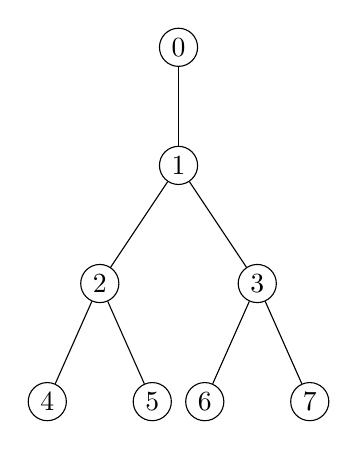
\begin{tikzpicture}[
        level/.style={sibling distance=40mm/#1},
        every node/.style={circle, draw, minimum size=1em, inner sep=2pt}
      ]

      \node {0}
      child {node {1}
        child {node {2}
          child {node {4}}
          child {node {5}}
        }
        child {node {3}
          child {node {6}}
          child {node {7}}
        }
      };

    \end{tikzpicture}
  \end{minipage}
  \hfill
  \begin{minipage}{0.6\textwidth}
    \centering
    \begin{equation}
      A =
      \begin{bmatrix}
        \gamma & \beta \\
        \beta & \alpha & \beta & \beta \\
        & \beta & \alpha & & \beta & \beta \\
        & \beta & & \alpha & & & \beta & \beta  \\
        & & \beta & & \gamma \\
        & & \beta & & & \gamma \\
        & & & \beta & & & \gamma \\
        &       & & \beta  & & &       & \gamma \\
      \end{bmatrix}.
    \end{equation}
  \end{minipage}\label{fig:figure}
\end{figure}

In this matrix, $\gamma$ is assigned to the root node and leave nodes, while $\alpha$ is assigned to the internal nodes. The edges connecting the nodes are represented by $\beta$.

We consider the $\ell$ type of nonzero element instead of $\ell$th nonzero element here. Note for node $i$, we define $2i$ as its left child and $2i+1$ as its right child. The function $c(j, \ell)$ can be defined as
\begin{equation}
  c(j, \ell) =
  \begin{cases}
    2j, & \text{if } \ell = 0 \text{ and } j < 2^{n-1},\\
    2j + 1, & \text{if } \ell = 1 \text{ and } j < 2^{n-1},\\
    j/2, & \text{if } \ell = 2 \text{ and } 2 \mid j,\\
    (j-1)/2, & \text{if } \ell = 3 \text{ and } 2 \nmid j,\\
    j, & \text{if } 4 \leq \ell \leq 7.
  \end{cases}\label{eq:equation17}
\end{equation}

Multiply or divide by 2 is equivalent to a left or right shift operation. This is easy to implement with swap gates. For example, if we divide $[0j_2j_1j_0]$ by 2,
\begin{equation}
  [0j_2j_1j_0] \xrightarrow{\text{swap}(j_0,j_1)} [0j_2j_0j_1] \xrightarrow{\text{swap}(j_0,j_2)} [0j_0j_2j_1] \xrightarrow{\text{swap}(j_0,0)} [j_00j_1j_2].
\end{equation}
Measurement on the first qubit may be needed. This gives a oracle between $\ket{0}$ and $\ket{j}$, and we denote it as $M_2$ and $D_2$. Use $L$ and $R$ defined in Eq.~\eqref{eq:equation14}, $O_C$ can be constructed similarly in fig.~\ref{fig:tree_oc}.

\begin{figure}[htbp]
  \centering
  \includegraphics{pdf/tree_oc}
  \caption{Oracle $O_C$ for binary tree matrices}
  \label{fig:tree_oc}
\end{figure}

The construction of the $O_A$ depends on how $O_C$ is constructed. We can still write $O_A$ as a series of controlled rotations: $\theta_0 = 2\arccos \beta$ by $\ell_2 =0$, $\theta_1 = 2\arccos (\alpha/ 4)$ by $(\ell_2, j_2) = (1,0)$, $\theta_2 = 2\arccos (\gamma/ 4)$ by $(\ell_2, j_2) = (1,1)$, and $\theta_3 = 2\arccos (\gamma/ 4 - \beta/2) - \theta_1$ by $(\ell_2, j) = (1,0)$.

Combining the oracles $O_C$ and $O_A$, we get the complete quantum circuit for the block encoding of the extended binary tree matrix as shown in fig.~\ref{fig:tree_circuit}. This is the circuit for $8\times 8$ matrix, and can be easily extended to larger matrices by adding more qubits.

\begin{figure}[htbp]
  \centering
  \includegraphics{pdf/tree_circuit}
  \caption{Complete circuit for binary tree matrices.}
  \label{fig:tree_circuit}
\end{figure}

Just as discussed in the previous section, the number of each gate in the circuit is $\mathcal{O}(\log s)$, and all gates can be decomposed into $\mathrm{poly}(n)$ two-qubit controlled gates, and still, this algorithm is considered efficient.

\section{Efficient Block Encoding of Symmetric Stochastic Matrices without Scaling Factor}\label{sec:efficient-block-encoding-of-symmetric-stochastic-matrices-without-scaling-factor}
In the previous section, we introduced the general framework for constructing block encodings of $s$-sparse matrices in original paper.
However, this framework requires the scaling factor $1/s$ to ensure that the block encoding is exact.
In some situations, such as conducting quantum walks, we need to block encode symmetric stochastic matrices without the scaling factor.
In this section, we will explore how to construct block encodings of symmetric stochastic matrices without the scaling factor, which is a significant extension of the original framework.
Also we will use the quantum circuit to construct the block encoding of a quantum walk operator, which is a common application of symmetric stochastic matrices in quantum computing.

Before we proceed, we need to introduce the quantum singular value transformation (QSVT), which can be viewed as a powerful framework that allows quantum circuits to implement polynomial transformations of the singular values of a matrix embedded in a unitary operator.
The proof of Theorem~\ref{thm:qsp} and can be found in Gilyén et al.'s paper~\cite{Gilyen2019}.

\begin{theorem}[Quantum Signal Processing, QSP]
  \label{thm:qsp}
  Let
  \begin{equation}
    U(t) =
    \begin{bmatrix}
      t              & \sqrt{1 - t^2} \\
      \sqrt{1 - t^2} & -t
    \end{bmatrix}.\label{eq:equation15}
  \end{equation}
  There exists a set of phase angles $\Phi_d \equiv \{\phi_0, \ldots, \phi_d\} \in \mathbb{R}^{d+1}$ so that
  \begin{equation}
    U_{\Phi_d}(t) \equiv e^{i\phi_0 Z} \prod_{j=1}^d \left[ U(t) e^{i\phi_j Z} \right] =
    \begin{bmatrix}
      p(t)                 & -q(t)\sqrt{1 - t^2} \\
      q^*(t)\sqrt{1 - t^2} & p^*(t)
    \end{bmatrix},\label{eq:equation16}
  \end{equation}
  if and only if $p(t)$ and $q(t)$ are complex valued polynomials in $t$ and satisfy
  \begin{enumerate}
    \item $\deg(p) \leq d$, $\deg(q) \leq d - 1$;
    \item $p$ has parity $d \bmod 2$ and $q$ has parity $d - 1 \bmod 2$;
    \item $|p(t)|^2 + (1 - t^2)|q(t)|^2 = 1$, $\forall t \in [-1, 1]$.
  \end{enumerate}
  When $d = 0$, $\deg(q) \leq -1$ should be interpreted as $q = 0$.

\end{theorem}

In the theorem above, if we choose $\Phi_d \equiv (\phi_0, \phi_1, \ldots, \phi_d)$ as:
\begin{equation}
  \phi_j =
  \begin{cases}
    \pi/4, & j = 0 \text{ or } d \\
    \pi/2, & j = 1, \ldots, d-1,
  \end{cases}
\end{equation}
then $p(t)$ is the $d$th degree Chebyshev polynomial of the first kind.

For a polynomial $p(t)$ satisfying the conditions in Theorem~\ref{thm:qsp}, we can construct a quantum circuit that implements the polynomial transformation of the singular values of a matrix embedded in a unitary operator using QSP and quantization.

\begin{theorem}[Quantum Singular Value Transformation, QSVT]
  Consider d-degree polynomial $ P(x) $ satisfying QSP conditions,$U_A$ is a $(1,a,0)$-block-encoding of matrix $A$, we have:\\
  - For even $ d $:
  \begin{equation}
    e^{i\tilde{\phi}_0 Z_\Pi} \prod_{j=1}^{d/2} \left[ U_A^\dagger e^{i\tilde{\phi}_{2j-1} Z_\Pi} U_A e^{i\tilde{\phi}_{2j} Z_\Pi} \right] =
    \begin{pmatrix}
      P^\diamondsuit(A) & * \\
      *                 & *
    \end{pmatrix}
  \end{equation}

  - For odd $ d $:
  \begin{equation}
    e^{i\tilde{\phi}_0 Z_\Pi} U_A e^{i\tilde{\phi}_1 Z_\Pi} \prod_{j=1}^{(d-1)/2} \left[ U_A^\dagger e^{i\tilde{\phi}_{2j} Z_\Pi} U_A e^{i\tilde{\phi}_{2j+1} Z_\Pi} \right] =
    \begin{pmatrix}
      P^\vartriangleright(A) & * \\
      *                      & *
    \end{pmatrix}
  \end{equation}
  where $ \tilde{\phi}_j = \phi_j + (-1)^j \pi/2 $ , $\Pi = \ket{0}\bar{0}\otimes I$ and $ Z_\Pi = 2\Pi - I $.

  The equations above give a $(1,a+1,0)$-block-encoding of the matrix $P(A)$.
  The query complexity of $U_A$ is $d+1$.

  \label{thm:qsvt}
\end{theorem}

\section{Hermitian block encoding}

The previous section \ref{sec:block_encoding} provides a general framework for constructing block encodings of $s$-sparse matrices, but the encoding unitary $U_A$ does not necessarily preserve the Hermitian property of the matrix $A$. We will show in this section that how to construct a Hermitian block encoding of a sparse Hermitian matrix $A$ using the quantum circuit in theorem~\ref{thm:main_result2}.

\begin{theorem}
  Suppose $A$ is a sparse Hermitian matrix of dimension $2^n$ with at most $s = 2^m$ non-zeros per column, with $m \leq n$. If a unitary $O_C$ satisfies
  \begin{equation}
    O_C \ket{\ell} \ket{j} = \ket{c(j, \ell)} \ket{j},
  \end{equation}
  where $c(j, \ell)$ is the row index of the $\ell$th non-zero element in the $j$th column, and if there exists a unitary $O_A$ such that
  \begin{equation}
    (I \otimes O_A) \ket{0} \ket{0} \ket{i} \ket{j} = \ket{0} \left( \sqrt{|A_{ij}|} \ket{0} + \sqrt{1 - |A_{ij}|} \ket{1} \right) \ket{i} \ket{j},
  \end{equation}
  for $A_{ij} = |A_{ij}| e^{i \theta_{ij}}$, where $\theta_{ij} \in [0, 2\pi)$, the square root is uniquely defined as $\sqrt{A_{ij}} = \sqrt{|A_{ij}|} e^{i \theta_{ij}/2}$. Then the unitary $U_A$ represented by the circuit shown in fig. ~\ref{fig:hermitian_encoding} is a Hermitian block encoding of $A$, where $D_s$ is a diffusion operator defined as
  \begin{equation}
    D_s \equiv I_2 \otimes \cdots \otimes
    \underbrace{H \otimes H \otimes \cdots \otimes H}_{m},
  \end{equation}
  and SWAP is a swap operator that swaps the last two $n$-qubit registers in fig. ~\ref{fig:hermitian_encoding} respectively.
  \label{thm:main_result2}
\end{theorem}

\begin{figure}[htbp]
  \centering
  \includegraphics{pdf/hermitian_circuit}
  \caption{Quantum circuit for the Hermitian block encoding of a sparse Hermitian matrix $A$}
  \label{fig:hermitian_encoding}
\end{figure}

\bibliographystyle{unsrt}
\bibliography{references}
\end{document}